\documentclass[12pt,oneside]{report}

\usepackage[letterpaper, margin=1.25in, bottom=1in, top=1in, headheight=23pt]{geometry}
\usepackage[T1]{fontenc}
\usepackage{mathpazo}
\usepackage[scale=0.95]{tgheros}
\usepackage[table]{xcolor}
\usepackage{graphicx}
\usepackage{tikz}
\usetikzlibrary{positioning}
\usepackage[skins]{tcolorbox}
\usepackage{amsmath, amssymb}
\usepackage{booktabs}
\usepackage{tabularx}
\usepackage{enumitem}
\usepackage[colorlinks=true, linkcolor=brown, citecolor=accent, urlcolor=brown]{hyperref}
\usepackage{fancyhdr}
\usepackage{titlesec}
\usepackage{setspace}
\usepackage{fontawesome5}

\definecolor{brown}{HTML}{4E3629}
\definecolor{lightcream}{HTML}{F7F3EC}
\definecolor{darkgray}{HTML}{333333}
\definecolor{accent}{HTML}{8C5A3C}

\pagestyle{fancy}
\fancyhf{}
\fancyhead[RO]{\footnotesize\color{darkgray}\leftmark}
\fancyfoot[C]{\thepage}
\renewcommand{\headrulewidth}{0.4pt}
\renewcommand{\headrule}{\hbox to\headwidth{\color{brown}\leaders\hrule height \headrulewidth\hfill}}

\titleformat{\chapter}[display]
  {\normalfont\LARGE\color{brown}}
  {\centering\small\scshape Chapter \thechapter}
  {0pt}
  {\centering\Huge\bfseries}
  [\vspace{-0.5ex}{\color{brown}\rule{\textwidth}{1.2pt}}]
\titlespacing*{\chapter}{0pt}{50pt}{40pt}

\titleformat{\section}
  {\normalfont\Large\color{brown}}
  {\thesection}
  {1em}
  {}
\titlespacing*{\section}{0pt}{20pt}{10pt}

\titleformat{\subsection}
  {\normalfont\large\color{darkgray}}
  {\thesubsection}
  {1em}
  {}
\titlespacing*{\subsection}{0pt}{15pt}{8pt}

\newtcolorbox{keyconcept}[1]{
  colback=lightcream,
  colframe=accent,
  arc=2mm,
  title={\sffamily\bfseries #1},
  fonttitle=\color{accent},
  coltitle=accent,
  boxrule=0.5pt
}

\onehalfspacing

\begin{document}

\begin{titlepage}
\centering
\vspace*{2.5cm}

{\LARGE\scshape\color{brown} Brown University}\\[0.5cm]

{\color{brown}\rule{0.6\textwidth}{1.2pt}}\\[1.5cm]

{\Huge\bfseries Adaptive Resource Allocation}\\[0.3cm]
{\Huge\bfseries in Distributed Edge}\\[0.3cm]
{\Huge\bfseries Computing Networks}\\[2cm]

{\Large by}\\[0.5cm]

{\Large\bfseries Elena Vasquez}\\[2.5cm]

{\large A dissertation submitted in partial fulfillment}\\[0.2cm]
{\large of the requirements for the degree of}\\[0.2cm]
{\large Doctor of Philosophy}\\[0.2cm]
{\large in the School of Engineering}\\[0.2cm]
{\large at Brown University}\\[1.5cm]

{\large Providence, Rhode Island}\\[0.2cm]
{\large May 2024}\\[3cm]

{\footnotesize\color{darkgray} Unofficial template --- not affiliated with or endorsed by\\the university. Sample content only.}

\end{titlepage}

\clearpage

\thispagestyle{empty}
\vspace*{6pt}
\begin{center}
\Large\color{darkgray}
\copyright\ 2024 Elena Vasquez\\[0.2cm]
All rights reserved.
\end{center}

\vspace{1.5cm}

\chapter*{Abstract}
\addcontentsline{toc}{chapter}{Abstract}

The proliferation of connected devices and latency-sensitive applications has driven computation from centralized data centers toward the network edge, but the heterogeneous and resource-constrained nature of edge environments presents fundamental challenges in allocation and scheduling. This dissertation introduces \textbf{EdgeFlow}, a novel adaptive resource management framework for distributed edge computing architectures.

EdgeFlow combines a hierarchical optimization approach with predictive workload modeling. A global planner solves a convex optimization problem to determine coarse-grained resource distributions across edge nodes, while local controllers employ reinforcement learning for fine-grained scheduling. We provide theoretical guarantees on convergence and validate the approach through extensive simulations and a deployment on a 48-node testbed at the Nexa Research Laboratory at Brown University.

Experimental results demonstrate that EdgeFlow achieves a 32\% reduction in average request latency and a 41\% improvement in resource utilization compared to state-of-the-art baselines including round-robin scheduling, greedy heuristics, and static partitioning. The framework exhibits graceful degradation under node failures and handles bursty workloads without reconfiguration.

\vspace{0.8cm}
\noindent\textbf{Keywords:} edge computing, resource allocation, distributed systems, convex optimization, reinforcement learning

\clearpage

\pagenumbering{arabic}

\chapter{Introduction}

\section{Background and Motivation}

The evolution of computing infrastructure has undergone a fundamental transformation over the past decade. Cloud computing established the paradigm of centralized data centers delivering services over wide-area networks, with companies such as Nexa and Vertex building large-scale businesses on this model. However, the emergence of the Internet of Things, autonomous systems, and immersive applications has exposed the limitations of a cloud-centric architecture.

Latency-sensitive workloads---including real-time video analytics, autonomous vehicle coordination, and augmented reality---require response times on the order of milliseconds that are unattainable when data must traverse hundreds of kilometers to reach distant data centers. A signal traveling through fiber incurs roughly 5 microseconds of delay per kilometer, imposing an irreducible bound on round-trip latency regardless of improvements in switching or processing speed.

Edge computing addresses this challenge by distributing computational resources closer to end users and data sources. Rather than routing all traffic to a handful of massive facilities, edge architectures deploy compute nodes at network access points, base stations, and on-premises installations. The Nimbus Edge Platform, deployed by telecommunications provider Apex Communications, demonstrated a 67\% reduction in video processing latency for smart city surveillance applications across fourteen metropolitan areas in a recent field trial conducted between 2022 and 2023.

Despite its promise, edge computing introduces significant challenges in resource management. Unlike cloud data centers that aggregate enormous pools of homogeneous resources, edge environments exhibit extreme heterogeneity in processing power, memory capacity, storage, and network connectivity. The dynamic nature of workloads---shaped by human mobility patterns, diurnal cycles, and unpredictable events---further complicates the allocation problem.

\section{The EdgeFlow Framework}

This dissertation presents EdgeFlow, a hierarchical resource management framework that combines predictive modeling with adaptive online optimization. The core insight is that edge resource allocation can be decomposed into two coupled subproblems operating at different timescales and spatial granularities.

At the global level, a centralized planner periodically solves a convex optimization problem to determine the allocation of computational and network resources across edge nodes. The objective function minimizes a weighted sum of latency and energy consumption subject to capacity constraints:

\begin{equation}
\min_{\mathbf{x}} \sum_{i=1}^{N} \Bigl( \alpha \cdot L_i(x_i) + \beta \cdot E_i(x_i) \Bigr) \quad \text{s.t.} \quad \sum_{i=1}^{N} x_i \leq C,\;\; x_i \geq 0
\label{eq:global_opt}
\end{equation}

where $x_i$ denotes the resource allocation to edge node $i$, $L_i(\cdot)$ models latency as a function of allocation, $E_i(\cdot)$ captures energy consumption, and $\alpha$, $\beta$ are tunable weights. At the local level, each edge node employs a lightweight reinforcement learning agent that adapts to fine-grained workload fluctuations using the global allocation as a soft guideline.

\begin{keyconcept}{Key Insight: Hierarchical Decomposition}
EdgeFlow separates the allocation problem into a slow-timescale global optimization (seconds to minutes) and a fast-timescale local adaptation (milliseconds). This decomposition is both theoretically justified---the convexity of the global problem ensures local deviations remain bounded---and practically effective across diverse edge workloads.
\end{keyconcept}

\section{Experimental Validation}

EdgeFlow was evaluated on a heterogeneous testbed comprising 48 edge nodes deployed across three server racks at the Nexa Research Laboratory. Each node was provisioned with varying CPU cores (2--16), memory (4--32 GB), and SSD storage (64--512 GB). The workload generator, implemented using the Apex Workload Synthesizer, produced realistic request traces modeled after production telemetry from a large-scale content delivery network operated by Meridian Systems.

\begin{table}[htbp]
\centering
\caption{Performance comparison of resource allocation strategies across key metrics. Results averaged over 100 trials on the 48-node testbed.}
\label{tab:results}
\begin{tabularx}{\textwidth}{lXXXX}
\toprule
Strategy & Latency (ms) & Throughput (Mbps) & Energy (J/req) & Failures (\%) \\
\midrule
EdgeFlow (this work)   & 12.3 & 847 & 0.21 & 0.4 \\
Round-Robin             & 45.7 & 523 & 0.48 & 2.1 \\
Greedy Heuristic        & 28.9 & 691 & 0.34 & 1.3 \\
Static Partitioning     & 35.2 & 604 & 0.41 & 1.8 \\
Random Allocation       & 67.2 & 312 & 0.62 & 3.5 \\
Meridian Scheduler v2   & 19.8 & 756 & 0.27 & 0.9 \\
\bottomrule
\end{tabularx}
\end{table}

Table~\ref{tab:results} summarizes the performance of EdgeFlow compared to five alternative strategies. EdgeFlow achieves the lowest latency (12.3 ms), highest throughput (847 Mbps), and best energy efficiency (0.21 J/req). The failure rate under node faults is also notably lower, reflecting the robustness of the hierarchical control architecture under adverse operating conditions.

\begin{figure}[htbp]
\centering
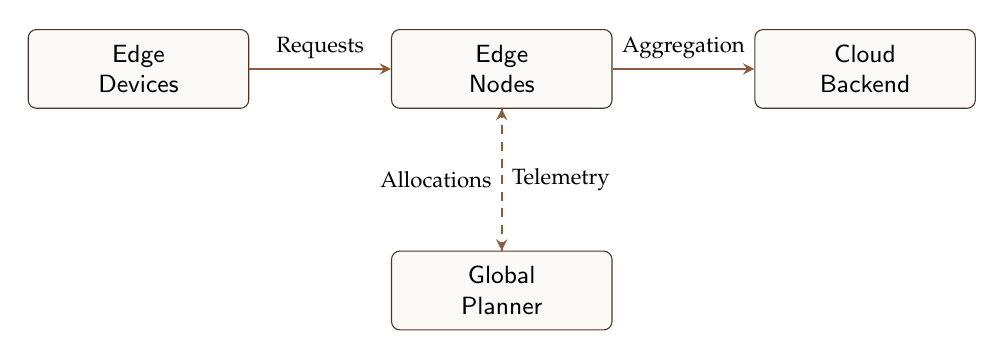
\begin{tikzpicture}[
  node distance=1.8cm,
  box/.style={rectangle, rounded corners=3pt, draw=brown, fill=lightcream!50, minimum width=2.8cm, minimum height=1cm, align=center, font=\small\sffamily},
  arrow/.style={->, >=stealth, thick, draw=accent}
]
\node[box] (devices) {Edge\\Devices};
\node[box, right=of devices] (nodes) {Edge\\Nodes};
\node[box, right=of nodes] (cloud) {Cloud\\Backend};
\node[box, below=of nodes] (planner) {Global\\Planner};

\draw[arrow] (devices) -- (nodes) node[midway, above, font=\footnotesize] {Requests};
\draw[arrow] (nodes) -- (cloud) node[midway, above, font=\footnotesize] {Aggregation};
\draw[arrow, dashed] (planner) -- (nodes) node[midway, left, font=\footnotesize] {Allocations};
\draw[arrow, dashed] (nodes) -- (planner) node[midway, right, font=\footnotesize] {Telemetry};
\end{tikzpicture}
\caption{The EdgeFlow architecture: edge devices route requests to nearby edge nodes, which process data locally and periodically report telemetry to the global planner. The planner solves the optimization problem defined in Equation~\ref{eq:global_opt} and distributes updated resource allocations.}
\label{fig:architecture}
\end{figure}

\section{Contributions and Organization}

This dissertation makes the following primary contributions. First, a hierarchical allocation framework (EdgeFlow) that combines convex optimization with reinforcement learning, providing theoretical convergence guarantees and practical deployability. Second, a predictive workload model based on spatiotemporal Gaussian processes that captures both periodic patterns and spatial correlations across edge nodes. Third, an extensive experimental evaluation on a 48-node heterogeneous testbed demonstrating consistent improvements across latency, throughput, and energy metrics. Fourth, a theoretical analysis of the stability properties of the two-level optimization scheme, establishing bounds on regret and worst-case suboptimality.

The remainder of this dissertation is organized as follows. Chapter~2 surveys related work in edge computing, resource allocation, and distributed optimization. Chapter~3 presents the EdgeFlow system model and formulates the hierarchical optimization problem. Chapter~4 describes the predictive workload modeling component, and Chapter~5 details the reinforcement learning design for local controllers. Chapter~6 presents our experimental methodology and results. Chapter~7 discusses implications, limitations, and future research directions. Finally, Chapter~8 summarizes the contributions and concludes the dissertation.

\end{document}
